\newpage
\subsection*{Task 4}

\subsubsection*{a) and b)}

\begin{figure}[h!]
  \centering
  \begin{subfigure}[b]{0.49\textwidth}
    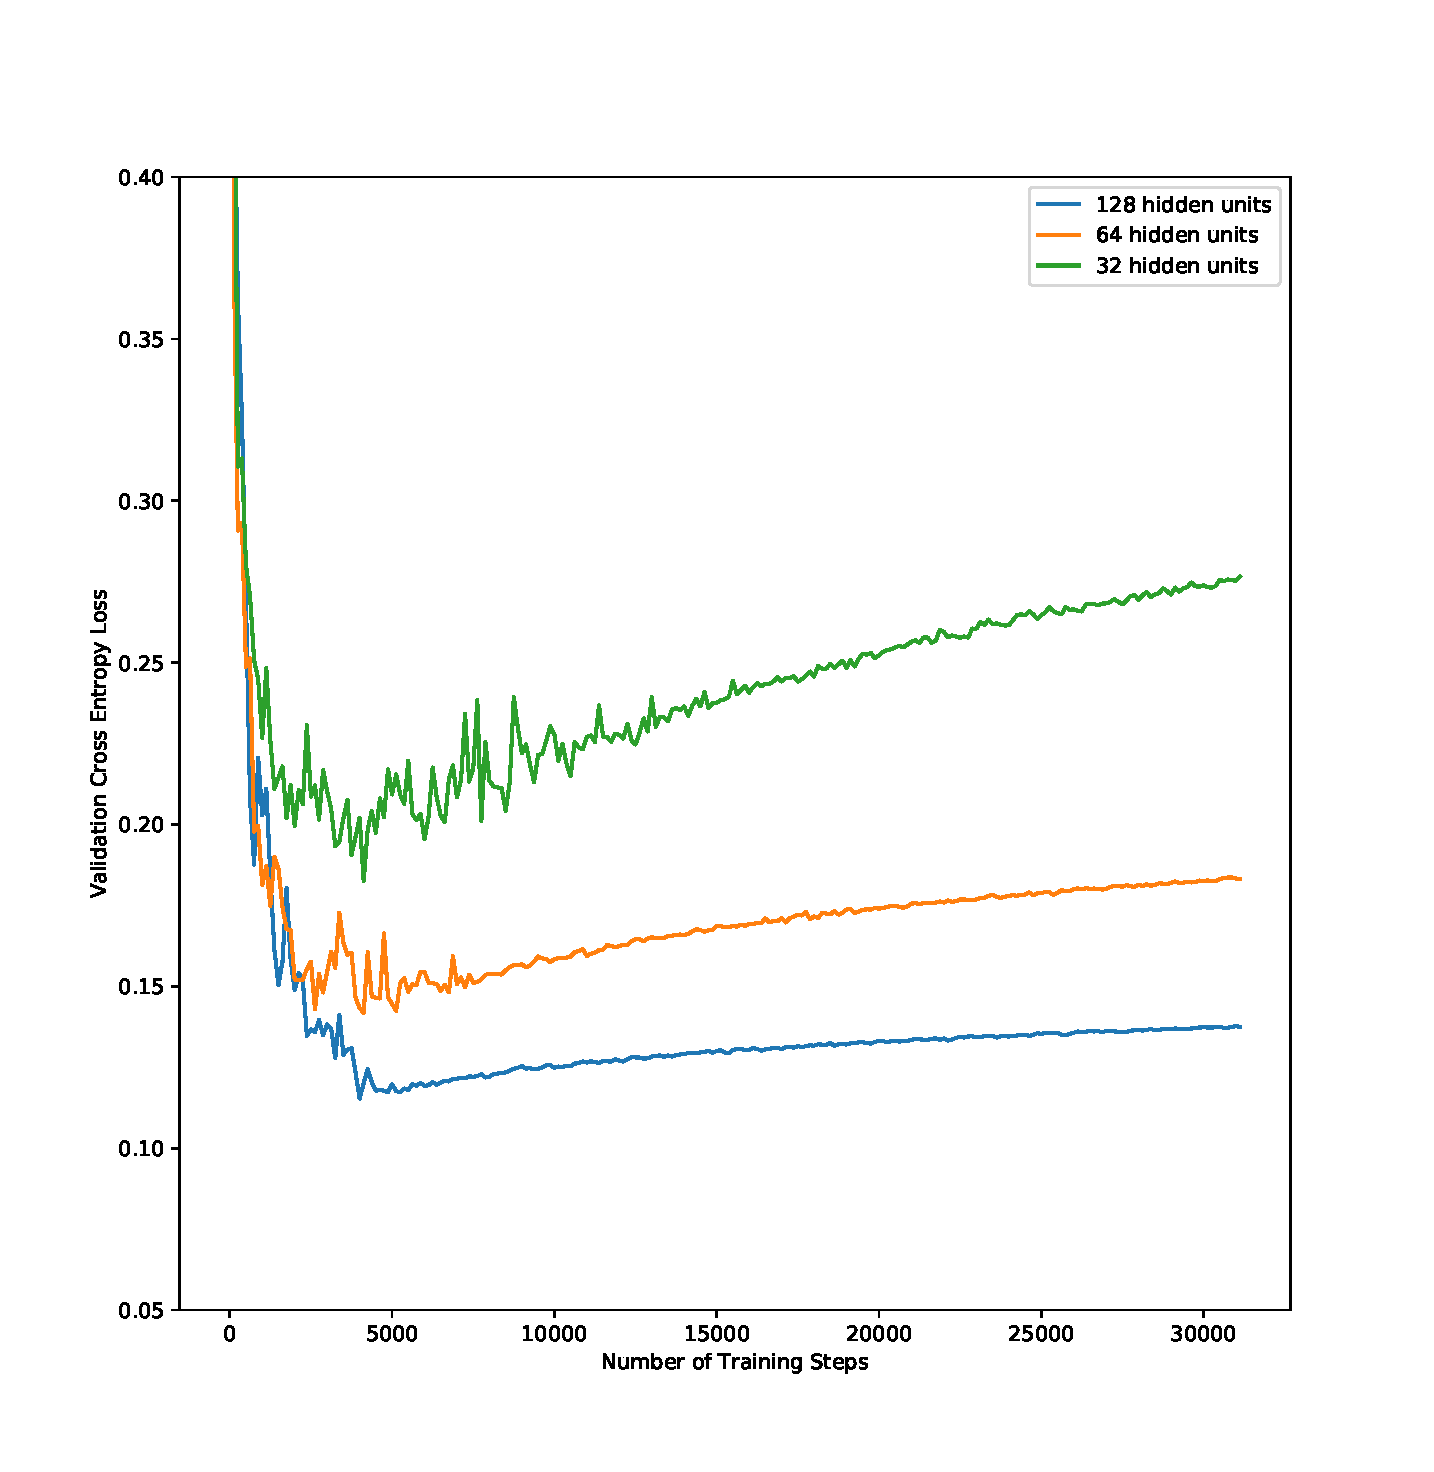
\includegraphics[clip,trim=1cm 0cm 1cm 0cm, width=\textwidth]{figures/Task4ab_loss.pdf}
    \caption{Loss with varying number of hidden units.}
  \end{subfigure}
 \hfill 
  \begin{subfigure}[b]{0.49\textwidth}
    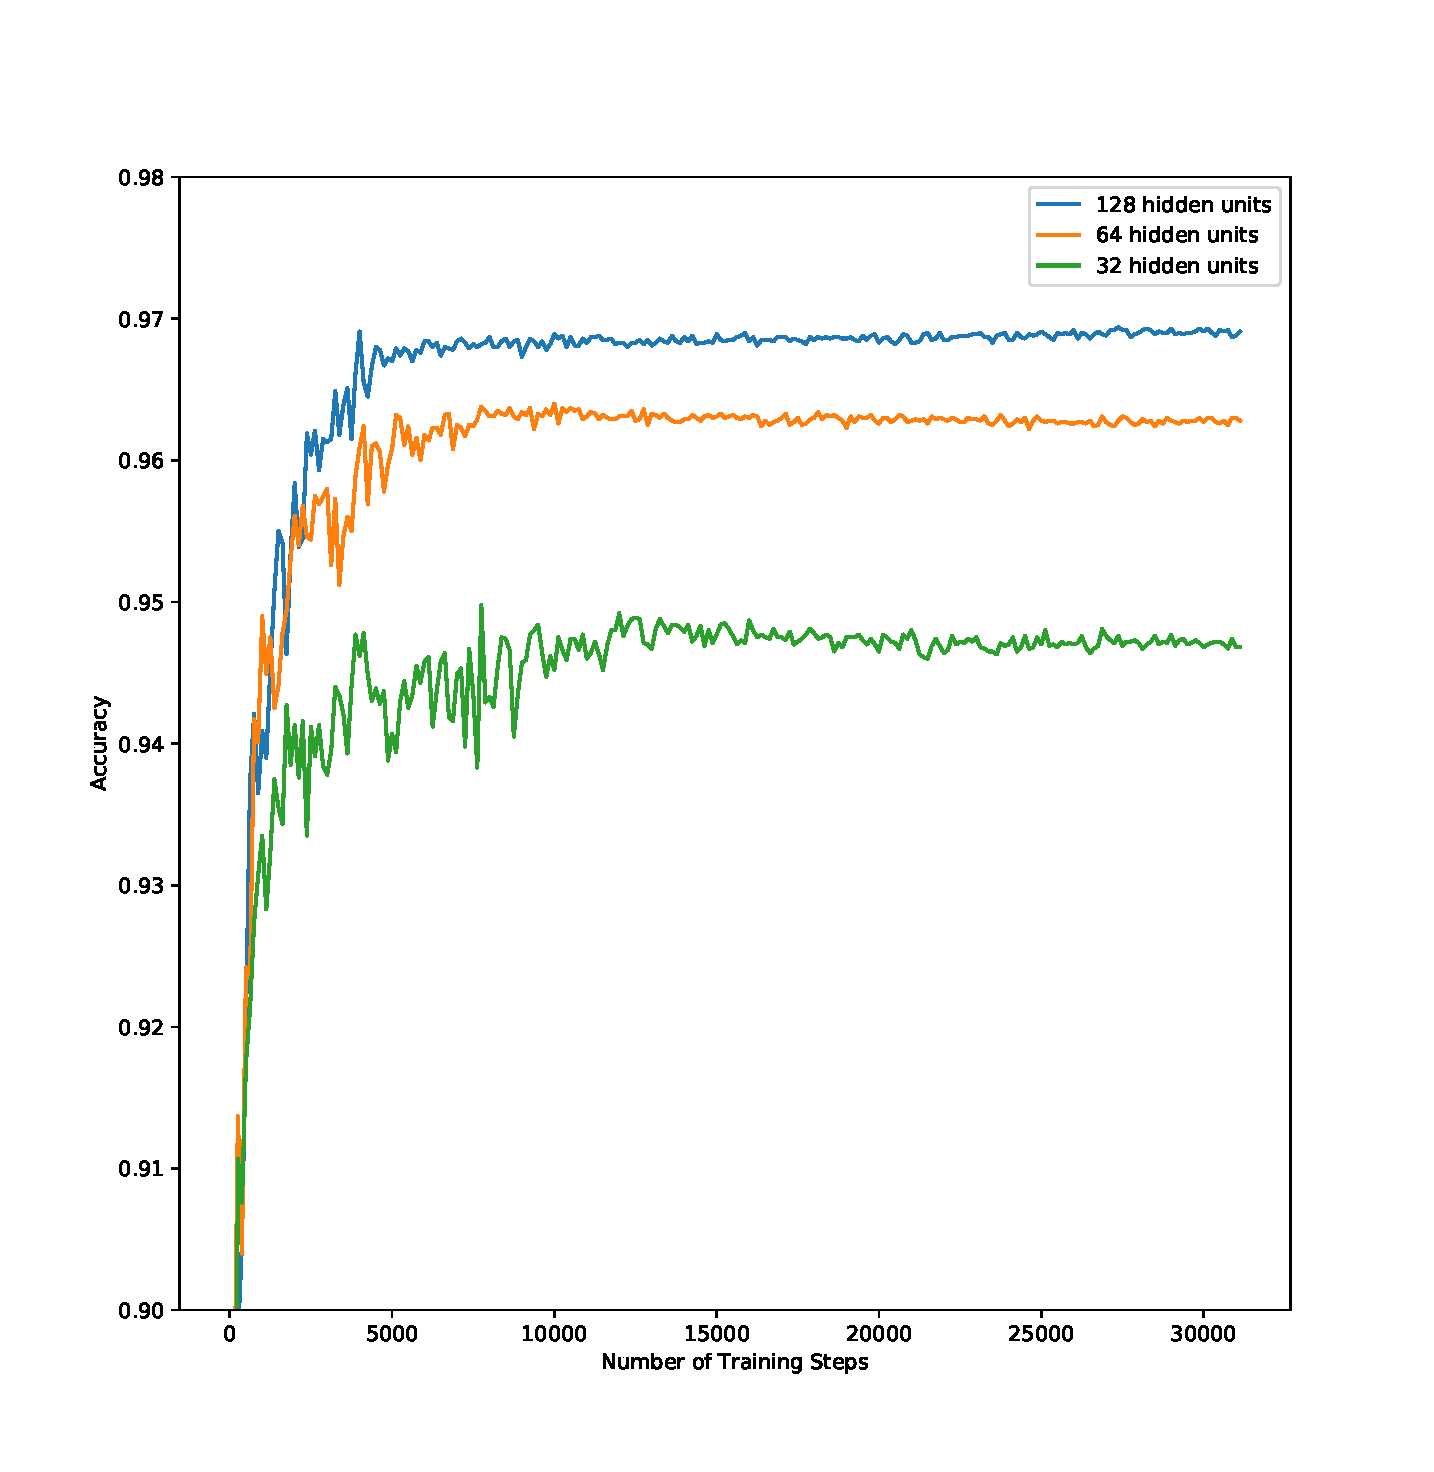
\includegraphics[clip,trim=1cm 0cm 1cm 0cm, width=\textwidth]{figures/Task4ab_accuracy.pdf}
    \caption{Accuracy with varying number of hidden units.}
  \end{subfigure}
  \caption{Validation set loss and accuracy over training with varying number of hidden units.}
  \label{fig:task4:ab}
\end{figure}

In \cref{fig:task4:ab} we see the results of using 128, 64 and 32 units in our hidden layer for the validation set. It seems that using too few units leads to slower convergence and poorer accuracy, meaning it might not be enough to capture the complexity of the underlying model. It is however much faster computationally. The network with 128 units performs quite well, giving the highest accuracy, but is also computationally most demanding by a large margin. The small increase in accuracy from the network with 64 units should therefore be weighed against the increase in computation time when choosing network topology.


\subsubsection*{d)}

From Task 3 we had 50880 parameters. To achieve around the same number of parameters with two hidden layers, we use 60 units in each hidden layer, so that the total number of parameters is $785 \times 60 + 60 \times 60 + 60 \times 10 = 51300$.

From \cref{fig:task4:d} we see that the network performs similarly to the one in Task 3, although the training takes much more time. The previous network is therefore preferred for this model. Overfitting is now also apparent from the plot of training and validation loss, where the training loss goes to zero while the validation loss increases after some time. 

\subsubsection*{e)}

In \cref{fig:task4:e} we see the comparison between a network with ten hidden layers of 64 neurons each, and a network with two hidden layers of 60 neurons each (same as baseline from Task 3). There are now $785\times 64 + 9\times 64\times 64 + 64\times 10=87744$ parameters in the network, so the network has a much higher complexity than before. This means a small change in input may give a large change in output, and we see from \cref{fig:task4:e} that the network zig-zags much more because of this, giving a much slower convergence. This is analogous to fitting a high order polynomial to a few points from an unknown model, which will heavily miss a new point. In the same way, the network overfits a batch while training, and when a new batch is given the network struggles to adapt to the new input.  

\begin{figure}[h!]
  \centering
  \begin{subfigure}[b]{0.49\textwidth}
    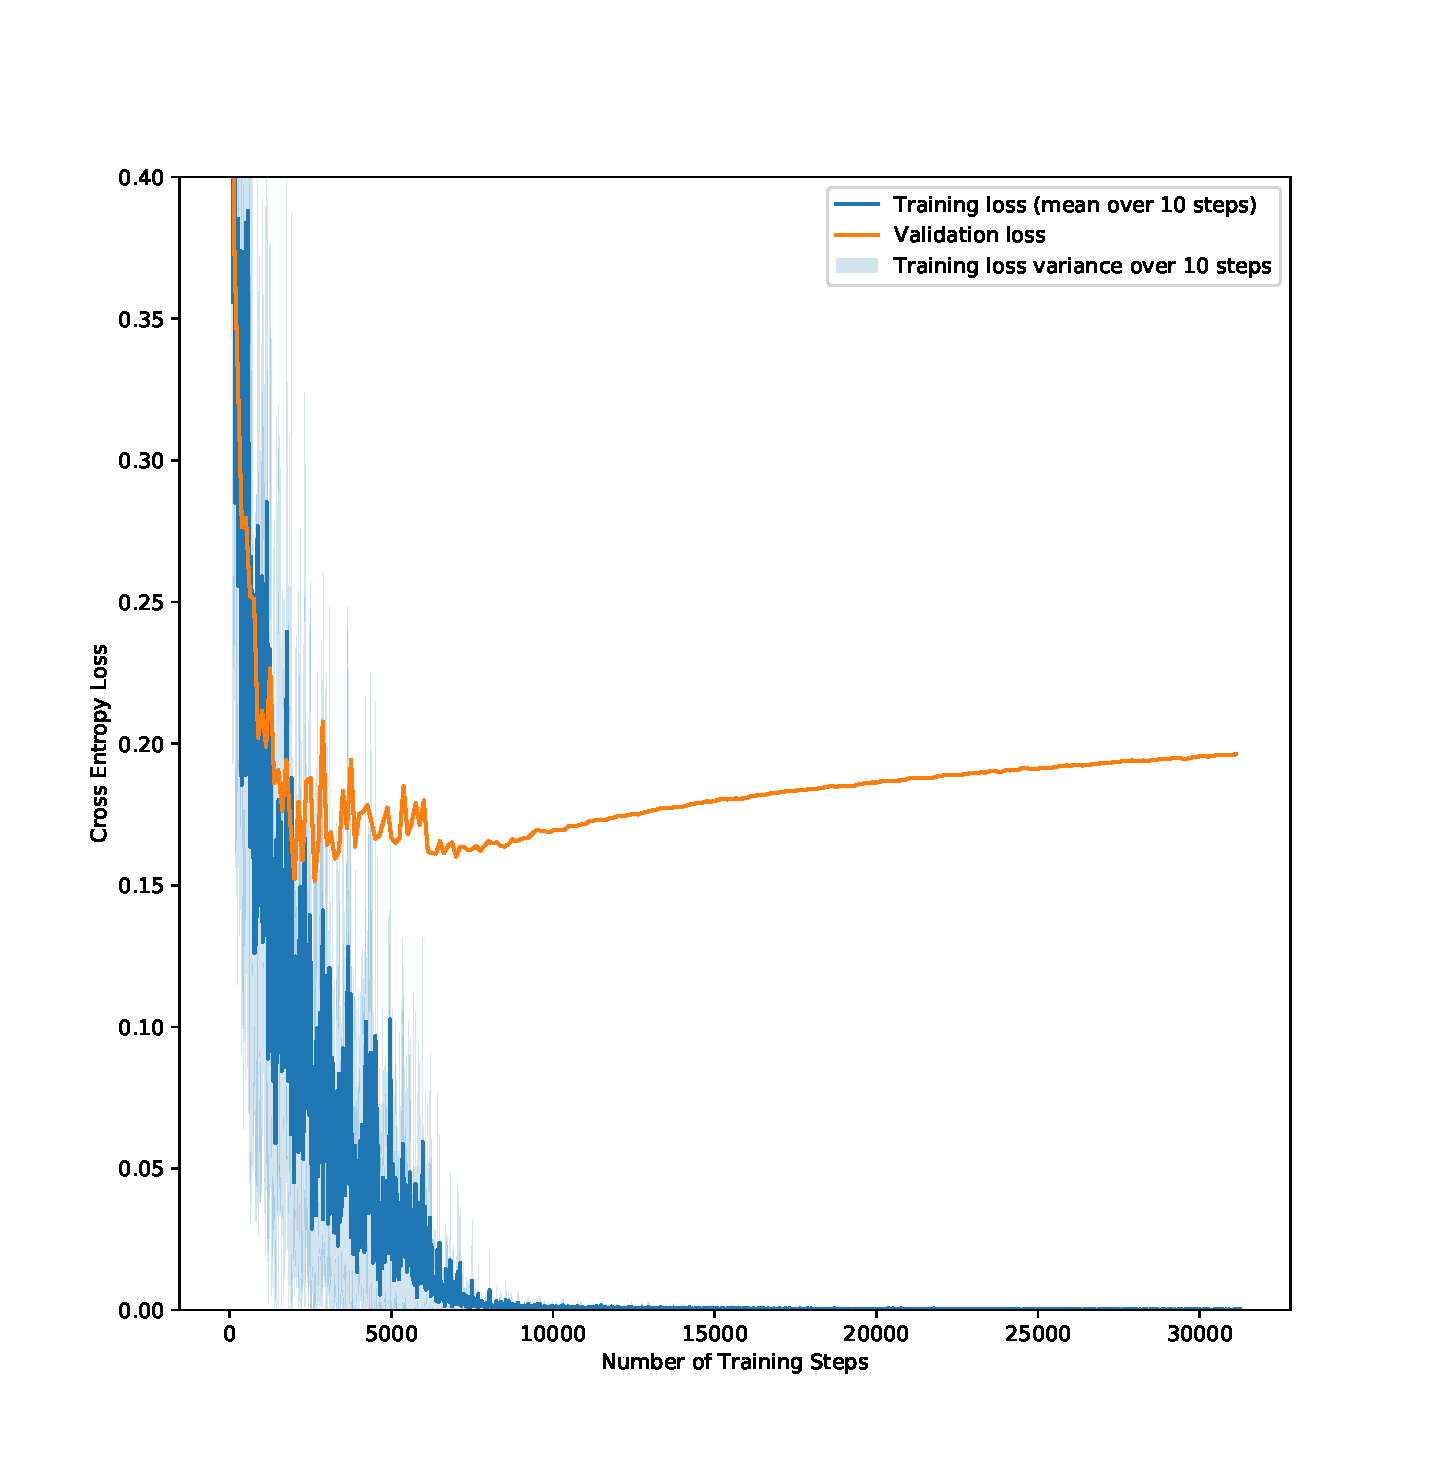
\includegraphics[clip, trim=1cm 0cm 1cm 0cm, width=\textwidth]{figures/Task4d_loss.pdf}
    \caption{Training and validation loss.}
  \end{subfigure}
  \hfill
  \begin{subfigure}[b]{0.49\textwidth}
    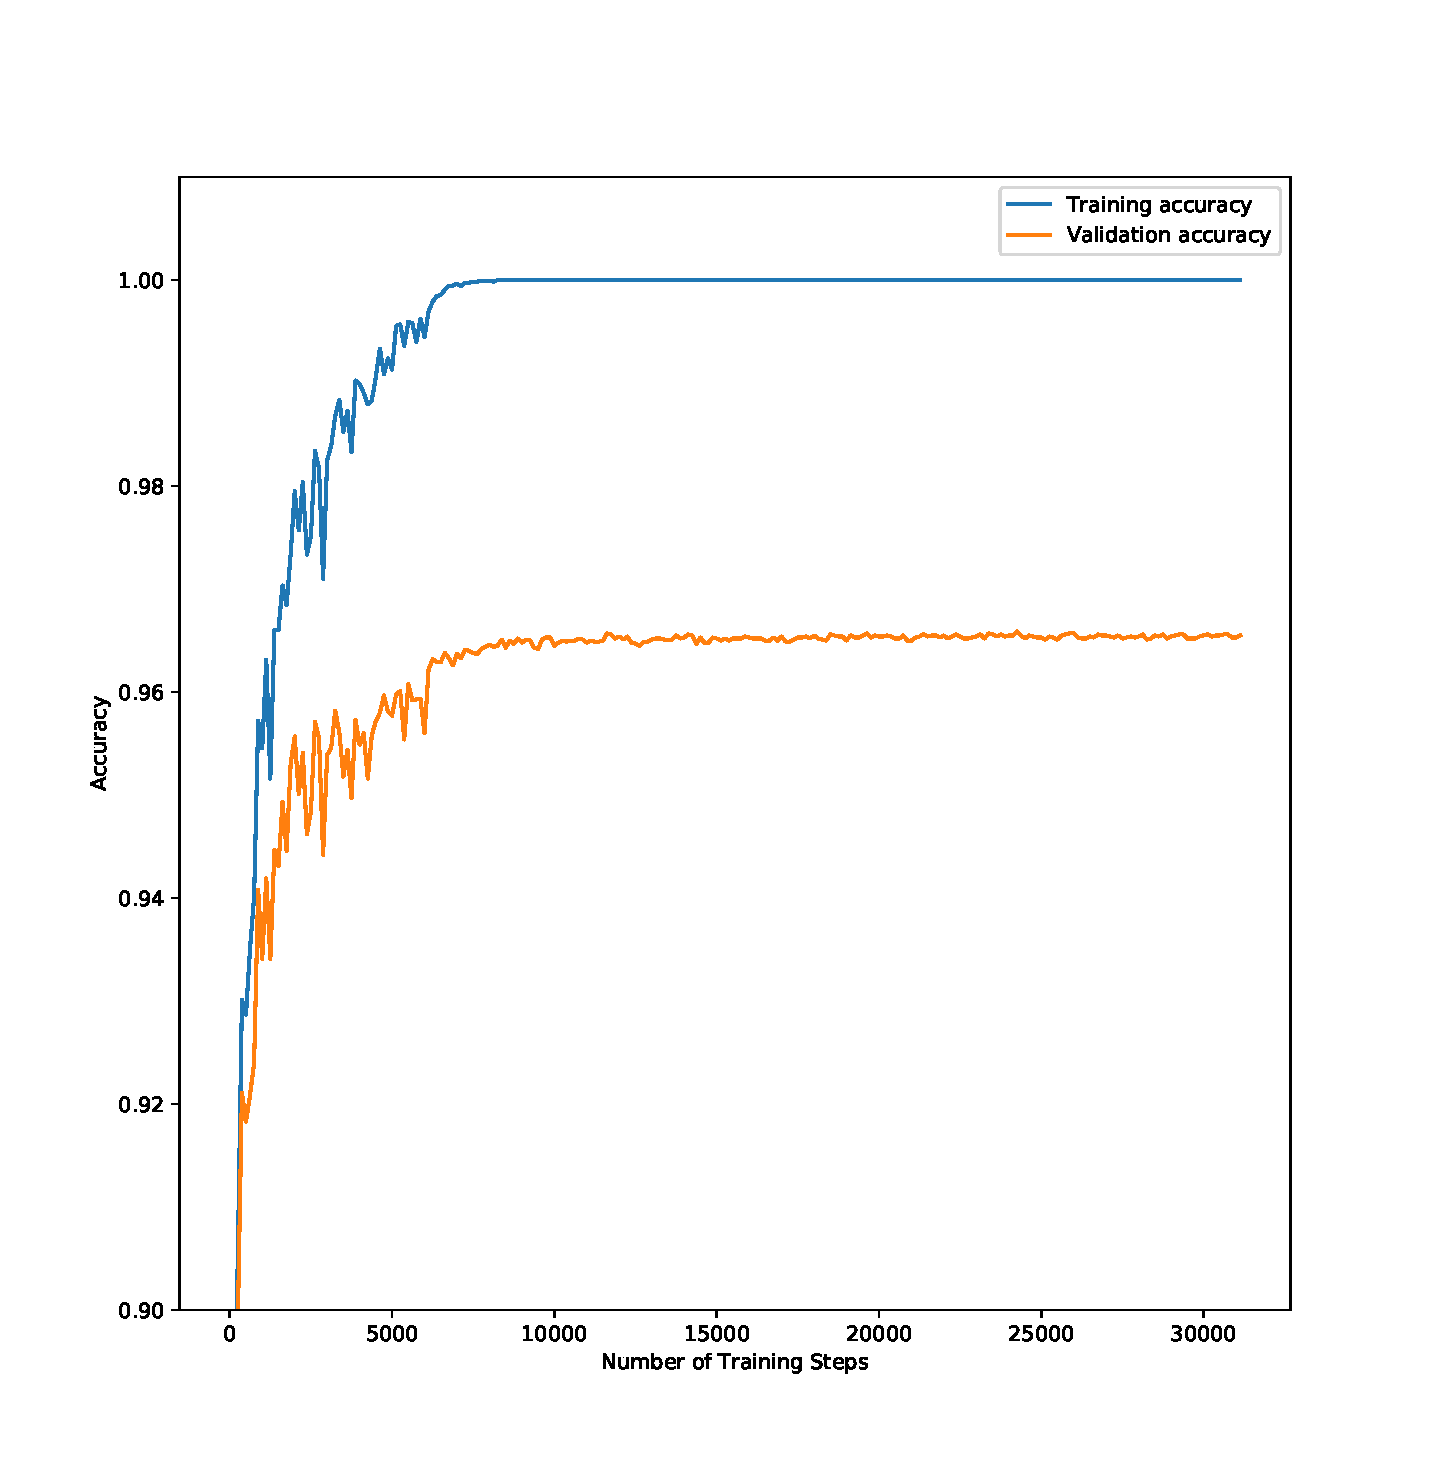
\includegraphics[clip, trim=1cm 0cm 1cm 0cm, width=\textwidth]{figures/Task4d_accuracy.pdf}
    \caption{Training and validation accuracy.}
  \end{subfigure}
  \caption{Cross entropy loss and accuracy with two hidden layers of 60 units each.}
  \label{fig:task4:d}
\end{figure}

\begin{figure}[h!]
  \centering
  \begin{subfigure}[b]{0.49\textwidth}
    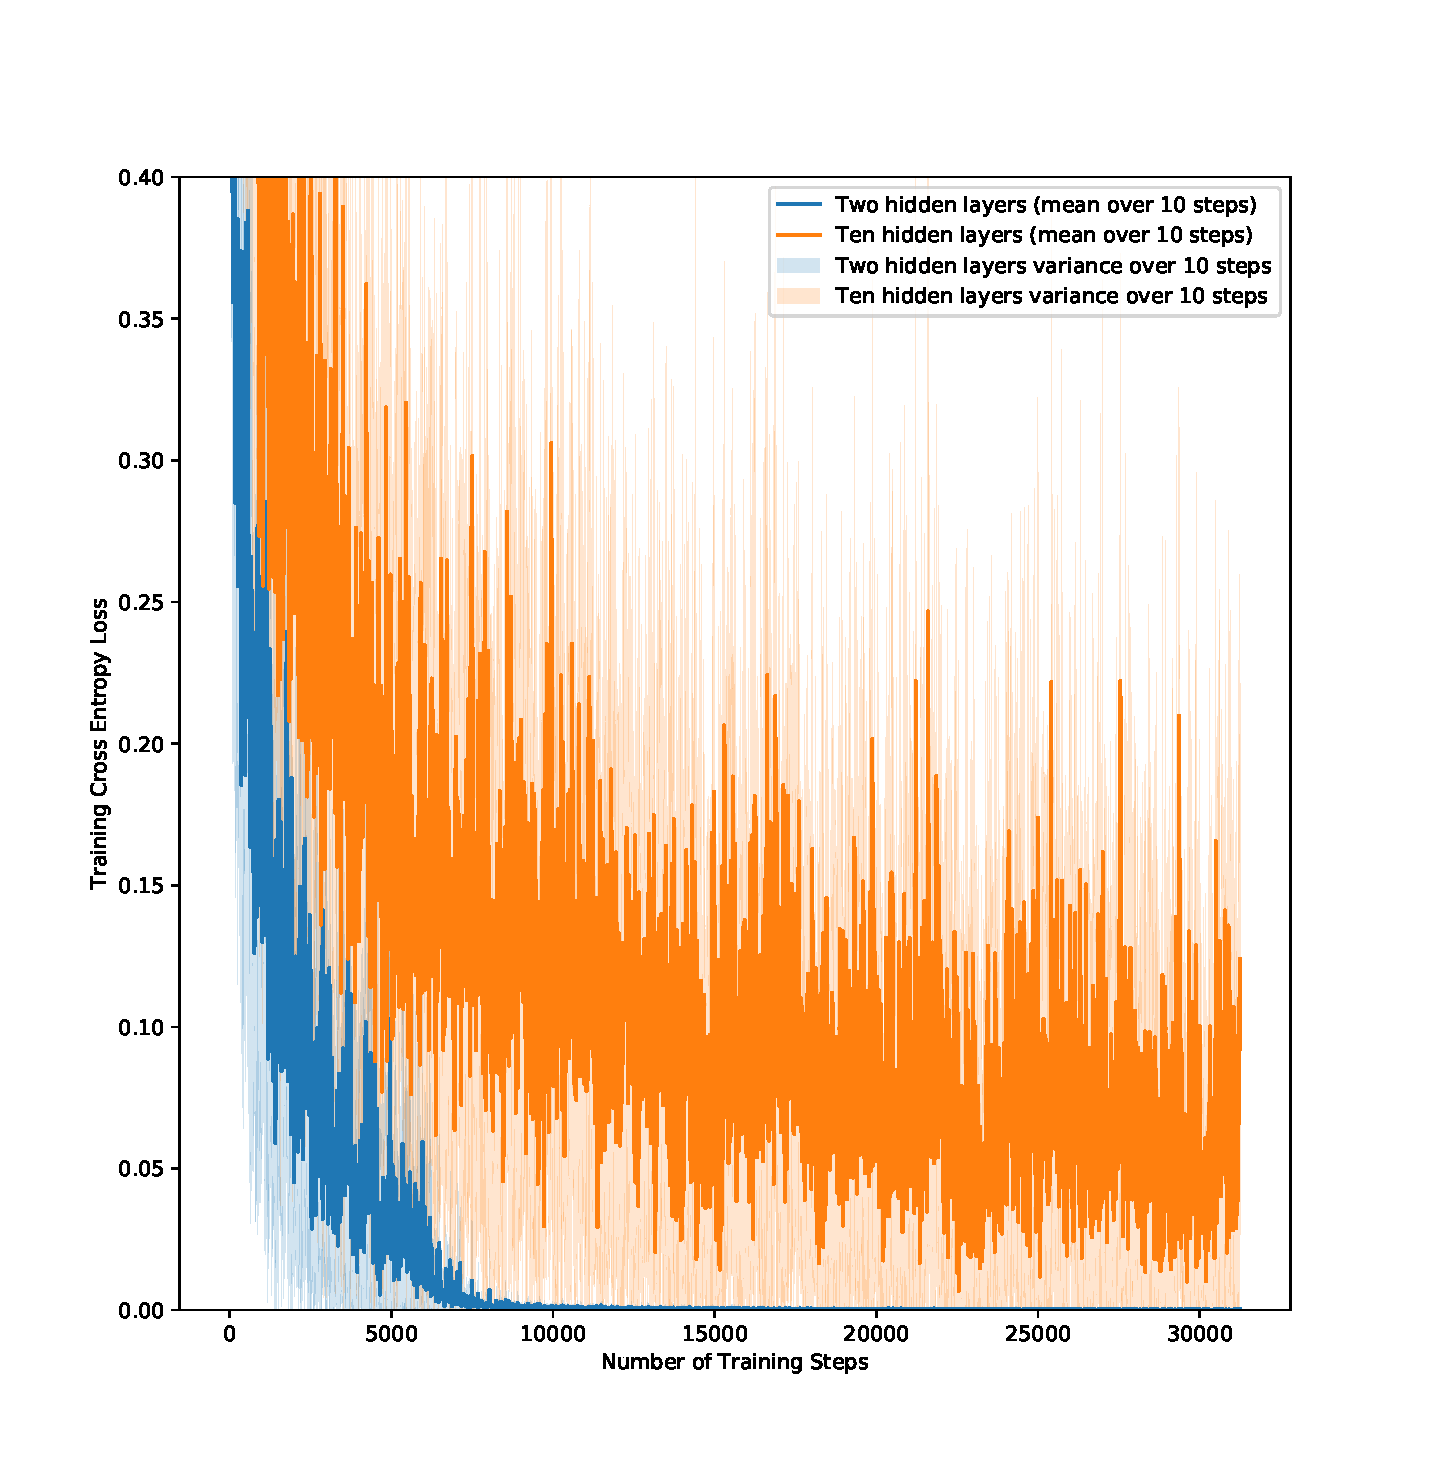
\includegraphics[clip, trim=1cm 0cm 1cm 0cm, width=\textwidth]{figures/Task4e_loss.pdf}
    \caption{Training loss.}
  \end{subfigure}
  \hfill
  \begin{subfigure}[b]{0.49\textwidth}
    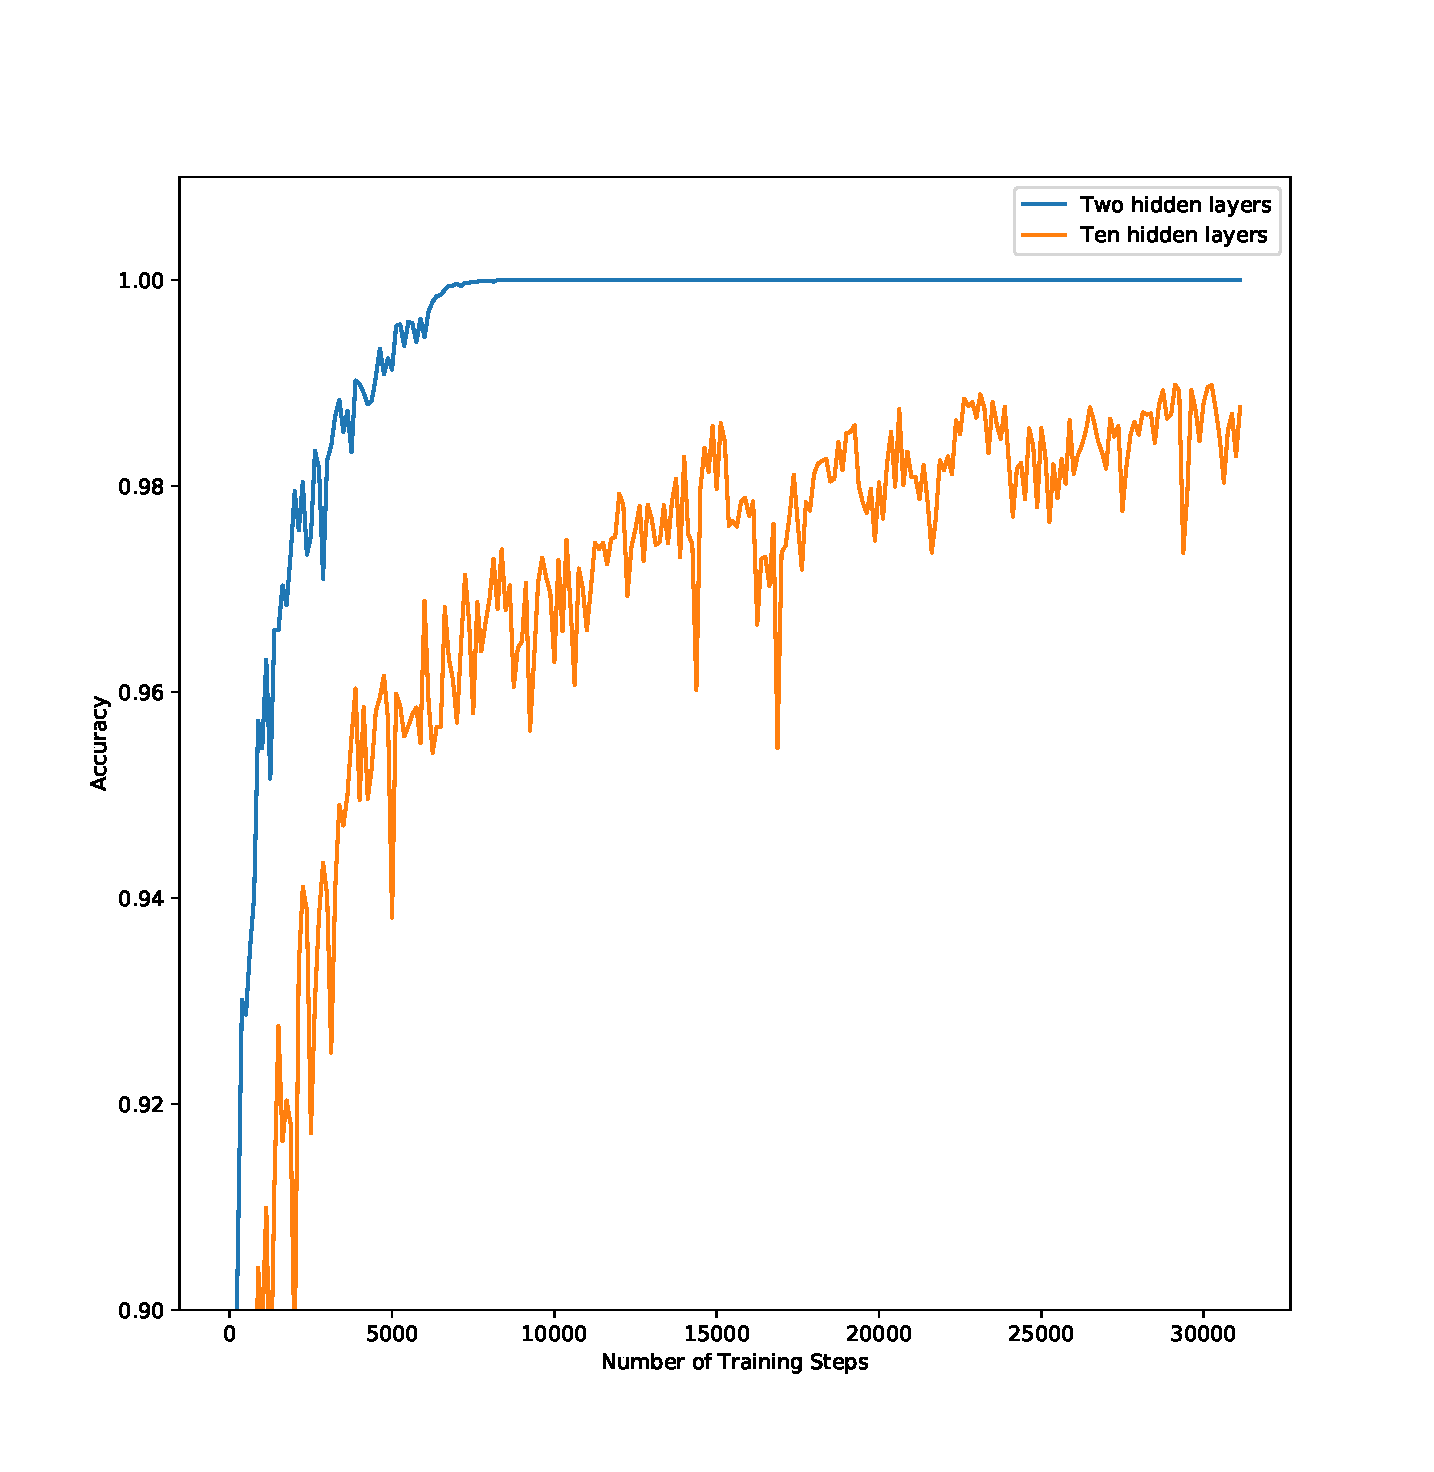
\includegraphics[clip, trim=1cm 0cm 1cm 0cm, width=\textwidth]{figures/Task4e_accuracy.pdf}
    \caption{Training accuracy.}
  \end{subfigure}
  \caption{Cross entropy loss and accuracy on training set for two different network topologies.}
  \label{fig:task4:e}
\end{figure}
